\documentclass{article}
\usepackage{xeCJK}
\usepackage{listings}
\usepackage{minted}
\usepackage{graphicx}

\setsansfont{Ubuntu}
\setmonofont{Ubuntu Mono}
\setCJKmainfont{Noto Sans CJK SC}
\setCJKsansfont{Noto Sans CJK SC}
\setCJKmonofont{Noto Sans CJK SC}

\begin{document}
	\section{实验一\ 进程的建立}
		\subsection{实验目的}
			学会通过基本的 Windows 或者 Linux 进程控制函数,由父进程创建子进程,并实现父子进程协同工作。

		\subsection{实验软硬件环境}
			\texttt{Linux version 5.13.0-40-generic (buildd@ubuntu) \\ gcc (Ubuntu 9.4.0-1ubuntu1~20.04.1) 9.4.0,GNU ld (GNU Binutils for Ubuntu) 2.34}

		\subsection{实验内容}
			创建两个进程,让子进程读取一个文件,父进程等待子进程读取完文件后继续执行,实现进程协同工作。进程协同工作就是协调好两个进程,使之安排好先后次序并以此执行,可以用等待函数来实现这一点。当需要等待子进程运行结束时,可在父进程中调用等待函数。

		\subsection{实验程序及分析}
			\inputminted[linenos,breaklines,tabsize=4]{c}{lib1/lib1.c}

			使用 \mintinline{c}{fork()} 函数创建子进程。

			若 \mintinline{c}{fork()} 函数返回值等于 \texttt{0},则说明此进程为子进程。子进程读取文件并输出到屏幕,然后退出。

			若 \mintinline{c}{fork()} 函数返回值大于 \texttt{0},则说明此进程为父进程,返回值为子进程 PID。父进程中使用 \mintinline{c}{waitpid()} 函数挂起,等待子进程运行结束。

		\subsection{实验截图}
			\begin{figure}[htbp]
				\centering
				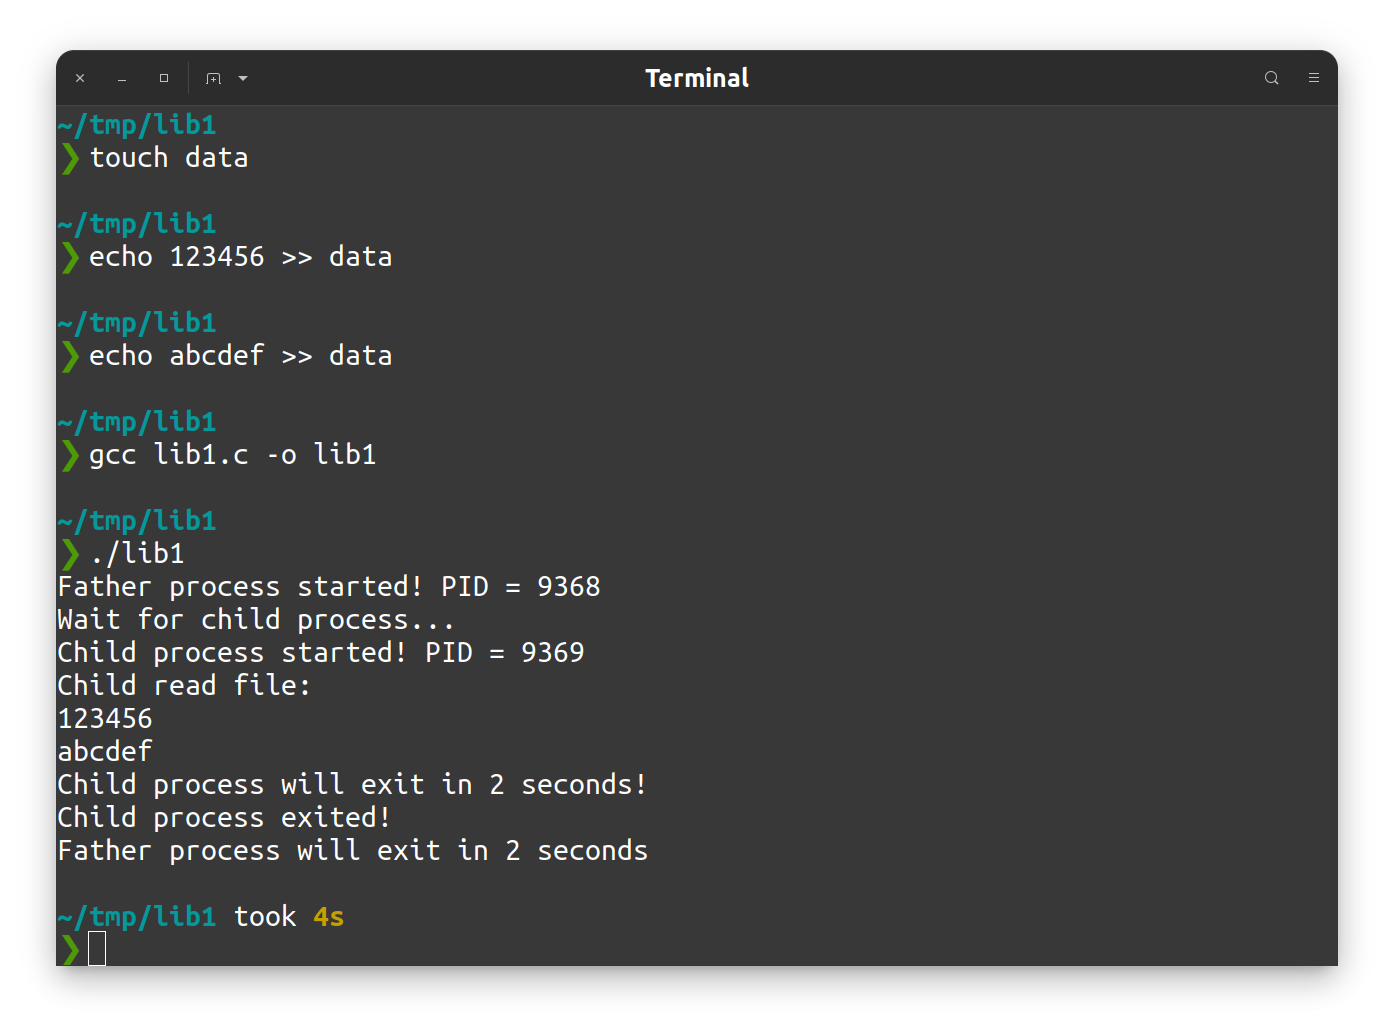
\includegraphics[width=\textwidth]{lib1/Screenshot.png}
				\caption{实验一\ 进程的建立}
			\end{figure}

		\subsection{实验心得体会}
			本次实验使用了 \mintinline{c}{fork()} 函数创建子进程,使用了 \mintinline{c}{waitpid()} 函数挂起父进程,达到父子进程协同工作的目的。通过实验,理解了进程的创建过程。

	\section{实验二\ 线程共享进程数据}
		\subsection{实验目的}
			了解线程与进程之间的数据共享关系。创建一个线程,在线程中更改进程中的数据。

		\subsection{实验软硬件环境}
			\texttt{Linux version 5.13.0-40-generic (buildd@ubuntu) \\ gcc (Ubuntu 9.4.0-1ubuntu1~20.04.1) 9.4.0,GNU ld (GNU Binutils for Ubuntu) 2.34}

		\subsection{实验内容}
			在进程中定义全局共享数据,在线程中直接引用该数据进行更改并输出该数据。

		\subsection{实验程序及分析}
			\inputminted[linenos,breaklines,tabsize=4]{c}{lib2/lib2.c}

			全局变量被进程和其子线程共享。故全局变量可被线程直接修改。

			使用 \mintinline{c}{pthread_create()} 函数创建线程。其中第三个参数是函数指针,表示线程执行函数。

			在进程中初始化全局共享变量并输出,然后在线程中修改全局共享变量并输出,最后等待线程函数执行完毕后,在进程输出全局共享变量。可以观察到线程成功修改了全局共享变量。

		\subsection{实验截图}
			\begin{figure}[htbp]
				\centering
				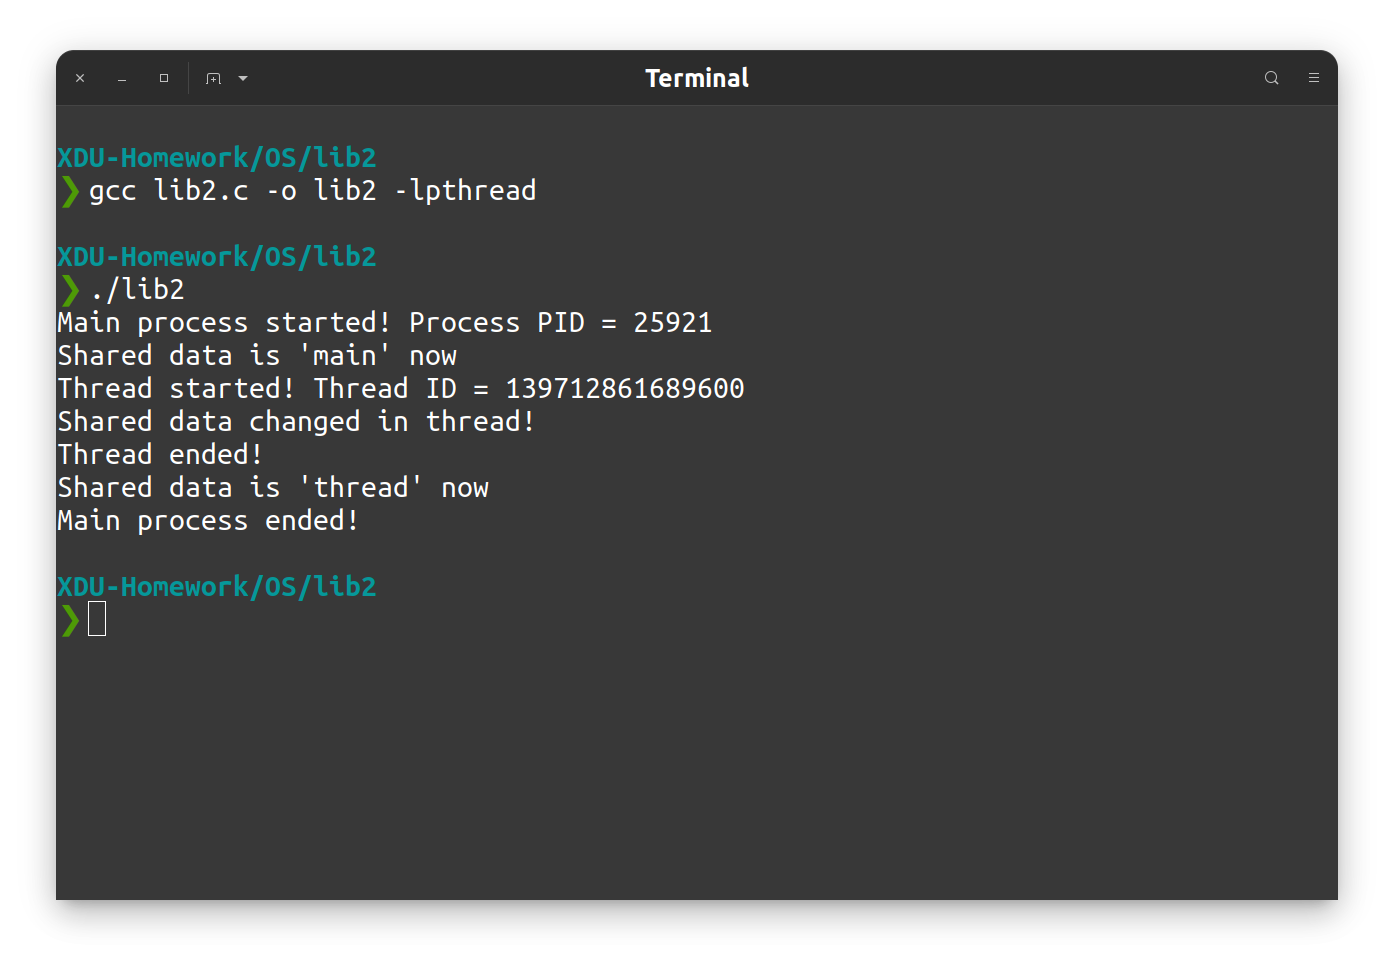
\includegraphics[width=\textwidth]{lib2/Screenshot.png}
				\caption{实验二\ 线程共享进程数据}
			\end{figure}

		\subsection{实验心得体会}
			本次实验使用了 \mintinline{c}{pthread_create()} 函数创建线程。并通过定义全局变量在进程和各个线程中共享,以达到线程通信的目的。通过本次实验,理解了如何定义全局共享变量,如何实现进程与线程之间的简单通信。

	\section{实验三\ 信号通信}
		\subsection{实验目的}
			利用信号通信机制在父子进程及兄弟进程间进行通信。

		\subsection{实验软硬件环境}
			\texttt{Linux version 5.13.0-40-generic (buildd@ubuntu) \\ gcc (Ubuntu 9.4.0-1ubuntu1~20.04.1) 9.4.0,GNU ld (GNU Binutils for Ubuntu) 2.34}

		\subsection{实验内容}
			父进程创建一个有名事件,由子进程发送事件信号,父进程获取事件信号后进行相应的处理。

		\subsection{实验程序及分析}
			\paragraph*{阻塞型通信}
				\inputminted[linenos,breaklines,tabsize=4]{c}{lib3/lib3_1.c}

				一个进程终止或者停止时,SIGCHILD 信号将被发送给其父进程。

				创建一个子进程,打印子进程 PID。子进程运行一段时间后退出。

				父进程调用信号处理函数 \mintinline{c}{signal()}, 捕获信号 SIGCHLD 并在 \mintinline{c}{handler()} 函数中处理。在 \mintinline{c}{handler()} 函数中输出退出的子进程的 PID。可以观察到,父进程成功捕获子进程的终止信号。

			\paragraph*{非阻塞型通信}
				\inputminted[linenos,breaklines,tabsize=4]{c}{lib3/lib3_2.c}

				在 Terminal 中按 \texttt{Ctrl + C} 可发送中断信号 SIGINT。

				父进程调用信号处理函数 \mintinline{c}{signal()}, 捕获信号 SIGINT 并在 \mintinline{c}{handler()} 函数中打印信息。

		\subsection{实验截图}
			\begin{figure}[htbp]
				\centering
				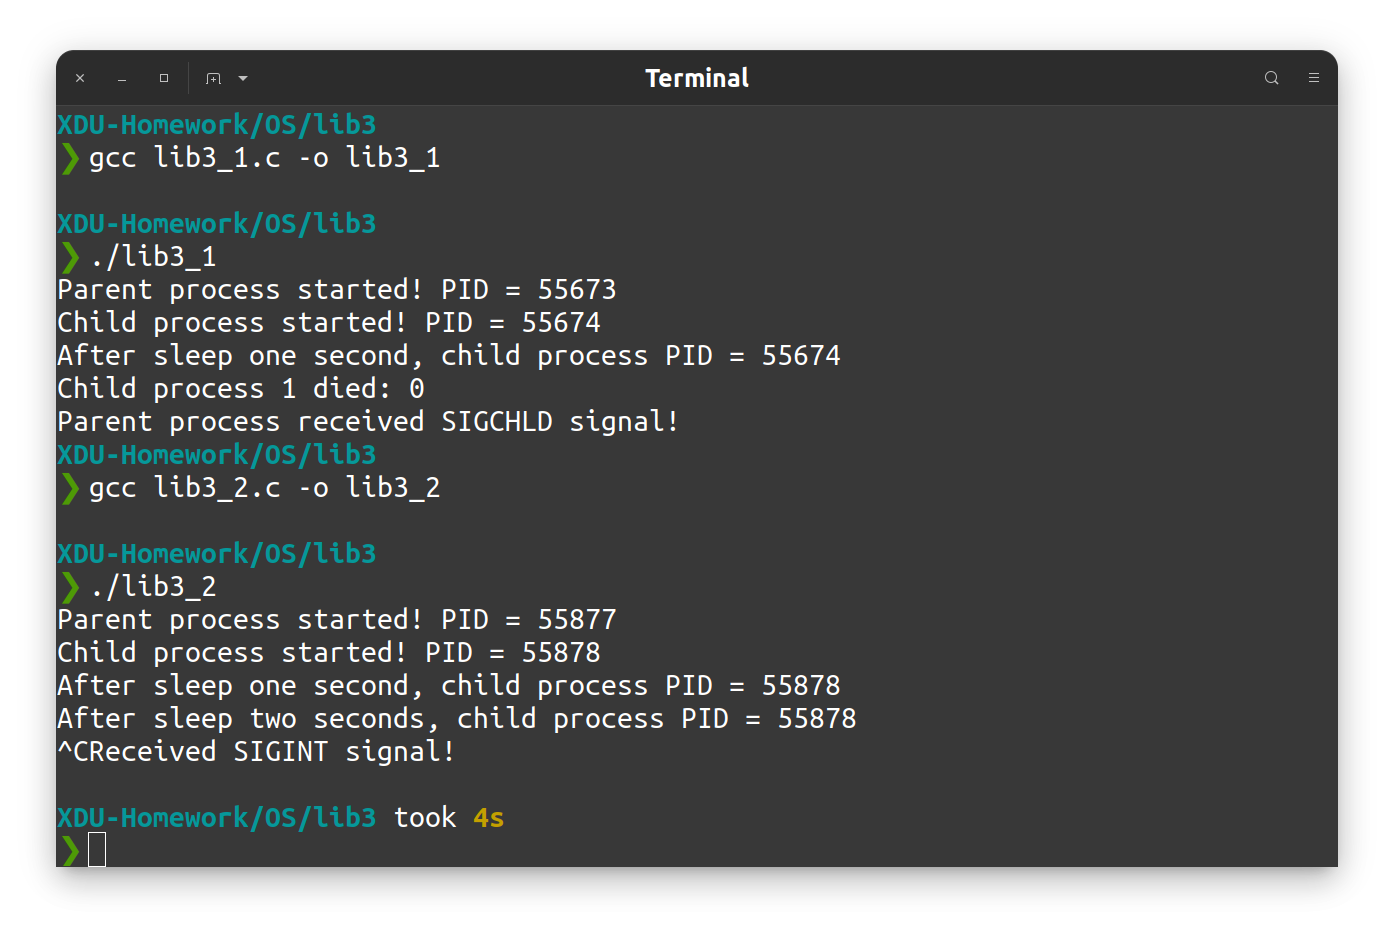
\includegraphics[width=\textwidth]{lib3/Screenshot.png}
				\caption{实验三\ 信号通信}
			\end{figure}

		\subsection{实验心得体会}
			本次实验使用了 \mintinline{c}{signal()} 函数捕获信号并做相应的处理。通过本次实验,理解了如何在进程之间进行信号通信。

	\section{实验四\ 匿名管道通信}
		\subsection{实验目的}
			学习使用匿名管道在两个进程间建立通信。

		\subsection{实验软硬件环境}
			\texttt{Linux version 5.15.0-30-generic (buildd@lgw01-amd64-058) \\ gcc (Ubuntu 11.2.0-19ubuntu1) 11.2.0, GNU ld (GNU Binutils for Ubuntu) 2.38}

		\subsection{实验内容}
			分别建立名为 Parent 的单文档应用程序和 Child 的单文档应用程序作为父子进程,由父进程创建一个匿名管道,实现父子进程向匿名管道写入和读取数据。

		\subsection{实验程序及分析}
			\inputminted[linenos,breaklines,tabsize=4]{c}{lib4/lib4.c}

			创建一个匿名管道,父子进程共享该管道。父进程向管道中写入数据,子进程从管道中读数据并输出。

		\subsection{实验截图}
			\begin{figure}[htbp]
				\centering
				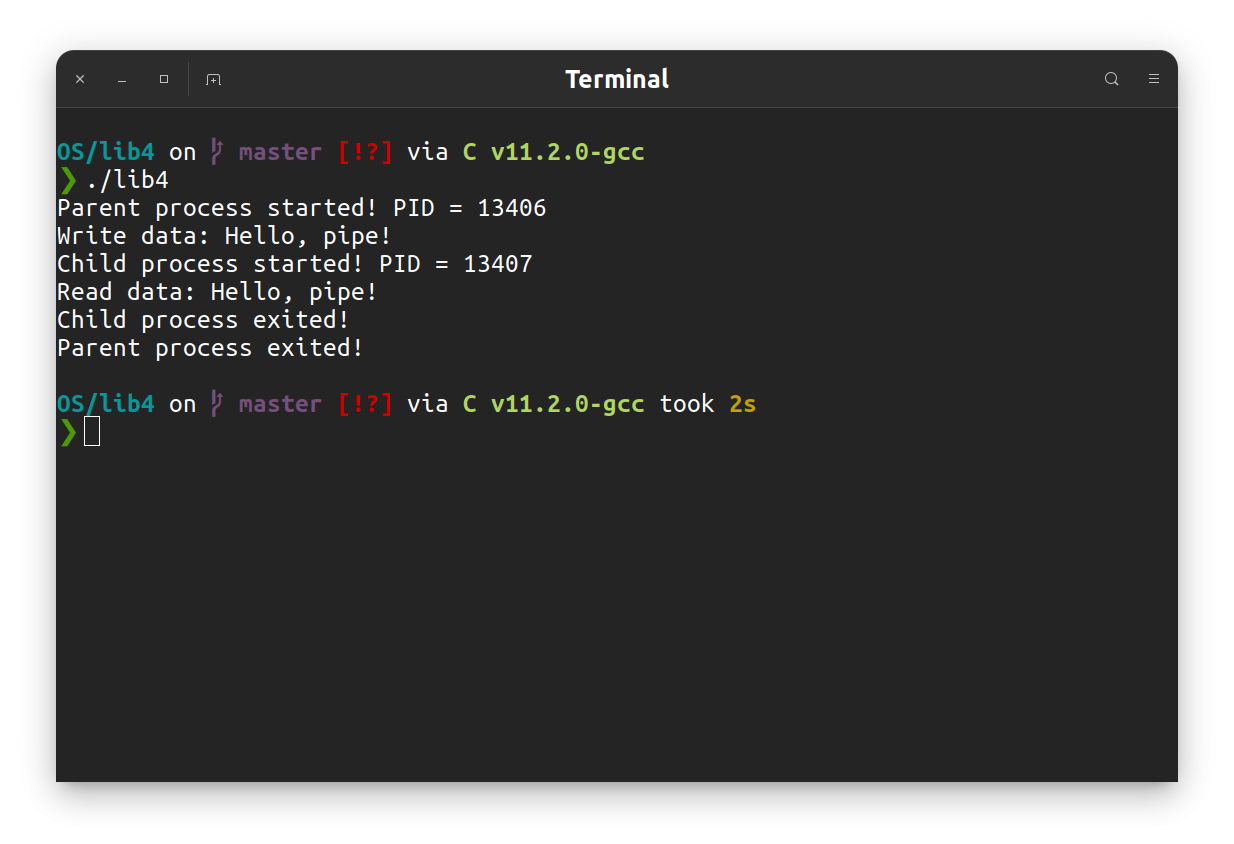
\includegraphics[width=\textwidth]{lib4/Screenshot.png}
				\caption{实验四\ 匿名管道通信}
			\end{figure}

		\subsection{实验心得体会}
			本次实验使用了 \mintinline{c}{pipe()} 函数创建匿名管道。通过父子进程共享数据实现管道通信。通过本次实验,理解了如何使用匿名管道进行通信。

	\section{实验五\ 命名管道通信}
		\subsection{实验目的}
			学习使用命名管道在多进程间建立通信。

		\subsection{实验软硬件环境}
			\texttt{Linux version 5.15.0-30-generic (buildd@lgw01-amd64-058) \\ gcc (Ubuntu 11.2.0-19ubuntu1) 11.2.0, GNU ld (GNU Binutils for Ubuntu) 2.38}

		\subsection{实验内容}
			建立父子进程,由父进程创建一个命名管道,由子进程向命名管道写入数据,由父进程从命名管道读取数据。

		\subsection{实验程序及分析}
			\inputminted[linenos,breaklines,tabsize=4]{c}{lib5/lib5.c}

			在当前目录下创建一个命名管道。子进程以写的方式打开命名管道,并向其中写入数据。父进程以读的方式打开命名管道,并从其中读取数据并输出。

			同时还可以观察到在当前目录下创建的命名管道文件。

			\newpage

		\subsection{实验截图}
			\begin{figure}[htbp]
				\centering
				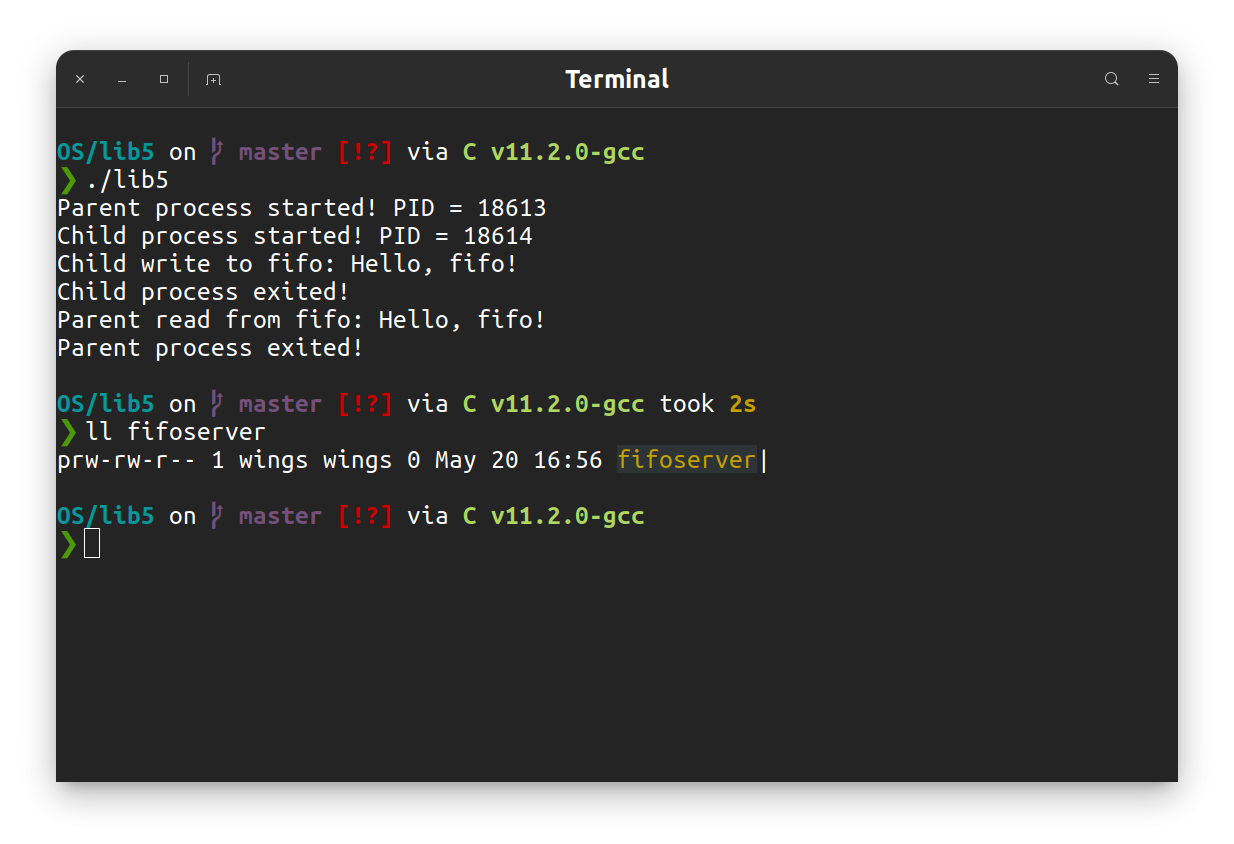
\includegraphics[width=\textwidth]{lib5/Screenshot.png}
				\caption{实验五\ 命名管道通信}
			\end{figure}

		\subsection{实验心得体会}
			本次实验使用了 \mintinline{c}{mkfifo()} 函数创建命名管道,利用命名管道实现进程间的通信。通过本次实验,理解了如何使用命名管道进行通信。

	\section{实验六\ 信号量实现进程同步}
		\subsection{实验目的}
			进程同步是操作系统多进程/多线程并发执行的关键之一,进程同步是并发进程为了完成共同任务采用某个条件来协调他们的活动,这是进程之间发生的一种直接制约关系。本次试验是利用信号量进行进程同步。

		\subsection{实验软硬件环境}
			\texttt{Linux version 5.15.0-30-generic (buildd@lgw01-amd64-058) \\ gcc (Ubuntu 11.2.0-19ubuntu1) 11.2.0, GNU ld (GNU Binutils for Ubuntu) 2.38}

		\subsection{实验内容}
			\begin{itemize}
				\item 生产者进程生产产品,消费者进程消费产品。
				\item 当生产者进程生产产品时,如果没有空缓冲区可用,那么生产者进程必须等待消费者进程释放出一个缓冲区。
				\item 当消费者进程消费产品时,如果缓冲区中没有产品,那么消费者进程将被阻塞,直到新的产品被生产出来。
			\end{itemize}

		\subsection{实验程序及分析}
			\inputminted[linenos,breaklines,tabsize=4]{c}{lib6/lib6.c}

			生产者先生产,当信号量 \mintinline{c}{empty} 为 0 时阻塞。待消费者开始消费,使得 \mintinline{c}{empty} 大于 0 后,生产者才可以继续生产。消费者将物品消费完后,信号量 \mintinline{c}{full} 为 0 时阻塞。等待生产者生产后,再唤醒并消费。同时,使用信号量 \mintinline{c}{mutex} 实现互斥锁,使得对生产者和消费者无法同时进入临界区对缓冲队列进行修改。

			\newpage

		\subsection{实验截图}
			\begin{figure}[htbp]
				\centering
				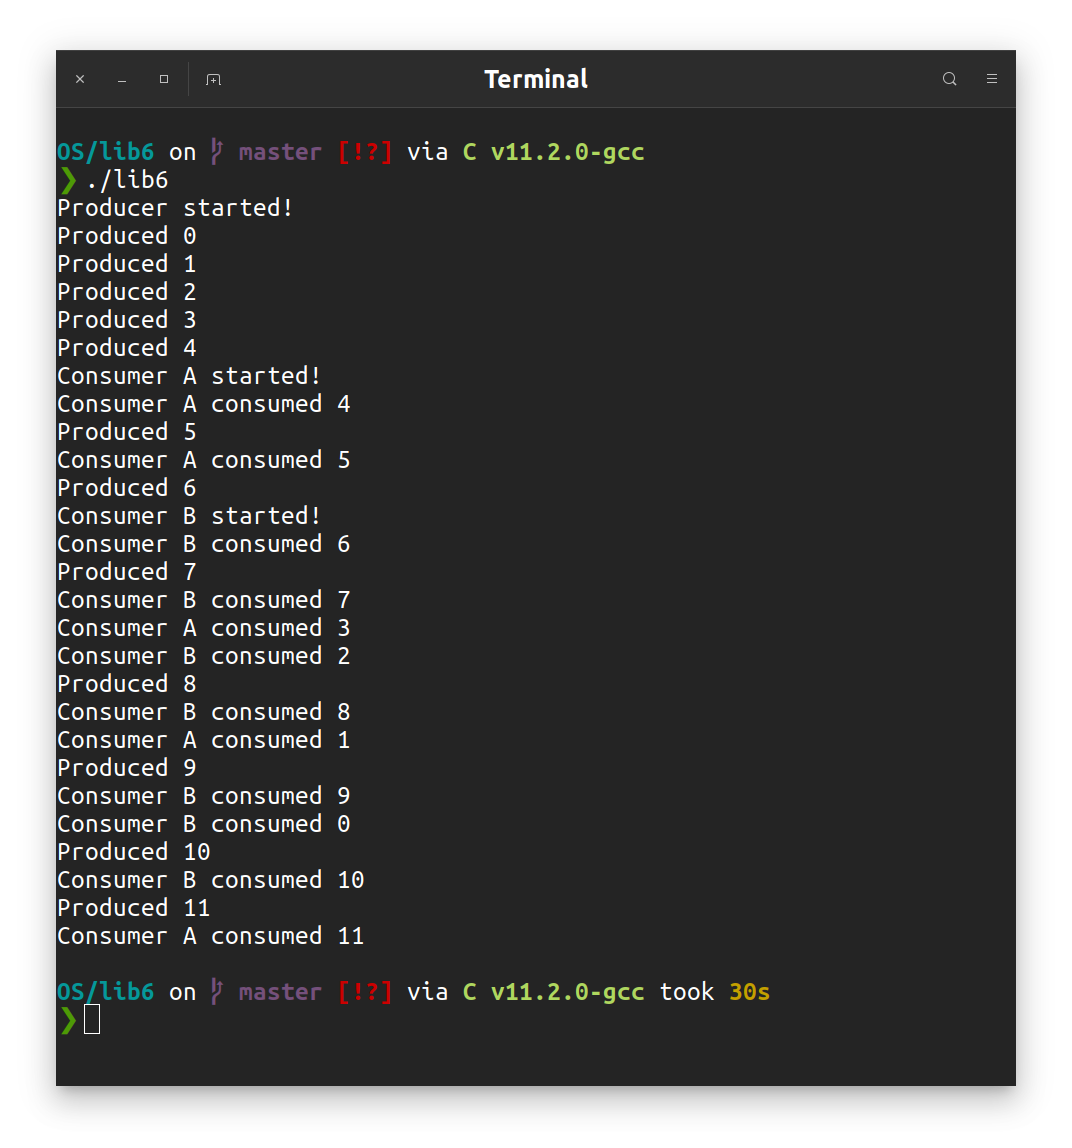
\includegraphics[width=\textwidth]{lib6/Screenshot.png}
				\caption{实验六\ 信号量实现进程同步}
			\end{figure}

		\subsection{实验心得体会}
			本次实验使用了信号量进行生产者与消费者的同步。通过本次实验,理解了如何使用信号量来进行同步。

\end{document}


